\documentclass[aspectratio=169]{beamer}
\usetheme{Madrid}
\usecolortheme{default}

\usepackage{booktabs}
\usepackage{graphicx}
\usepackage{array}

\title[Router Trajectories]{Gate Alignment Before Causal Branch Modularity}
\subtitle{Branch Specialization Phase 3 Toy Checkpoint}
\author{Branch specialization research project}
\date{2026-05-22}

\begin{document}

\begin{frame}
  \titlepage
  \vspace{-0.5em}
  \small
  Checkpoint reason: trajectory evidence identifies when role-informative
  routing pressure becomes causal branch modularity.
\end{frame}

\begin{frame}{Current Question}
  The annealed-label experiment showed that labels through step 400 fail, labels
  through step 800 partially persist, and labels through step 1200 persist more
  strongly.

  \vspace{0.8em}
  \textbf{Question.} What changes between step 400 and step 800?

  \vspace{0.8em}
  Two possibilities:
  \begin{itemize}
    \item the router gate itself may not be role-aligned until late;
    \item the gate may align early, while branch computations need more time to
    become causally separable.
  \end{itemize}
\end{frame}

\begin{frame}{Setup}
  \begin{itemize}
    \item Task: \texttt{bidirectional\_lookup}
    \item Branches: two 64-dim attention branches
    \item Seeds: 5
    \item Training: 1600 optimizer updates
    \item Trajectory steps: 0, 50, 100, 200, 400, 401, 600, 800, 801, 1000,
    1200, 1201, 1400, 1600
  \end{itemize}

  \vspace{0.5em}
  Conditions:
  \begin{center}
  \begin{tabular}{ll}
    \toprule
    Condition & Role-label schedule \\
    \midrule
    unlabeled & entropy 0.05 plus balance 1.0, no labels \\
    end 400 & weak labels for steps $<400$ \\
    end 800 & weak labels for steps $<800$ \\
    end 1200 & weak labels for steps $<1200$ \\
    always & weak labels for the full run \\
    \bottomrule
  \end{tabular}
  \end{center}
\end{frame}

\begin{frame}{Metric Glossary}
  \begin{description}
    \item[Gate role distance] Distance between local-role and induction-role
    router probability distributions. This measures where the gate sends tokens.
    \item[Gate routed match] Fraction of seeds where the gate maps local to
    branch 0 and induction to branch 1.
    \item[Causal branch distance] Distance between branch-use distributions
    inferred by branch ablation. This measures where the computation lives.
    \item[Routed causal match] Fraction of seeds where causal ablation maps
    local to branch 0 and induction to branch 1.
  \end{description}
\end{frame}

\begin{frame}{Trajectory Plot}
  \begin{center}
    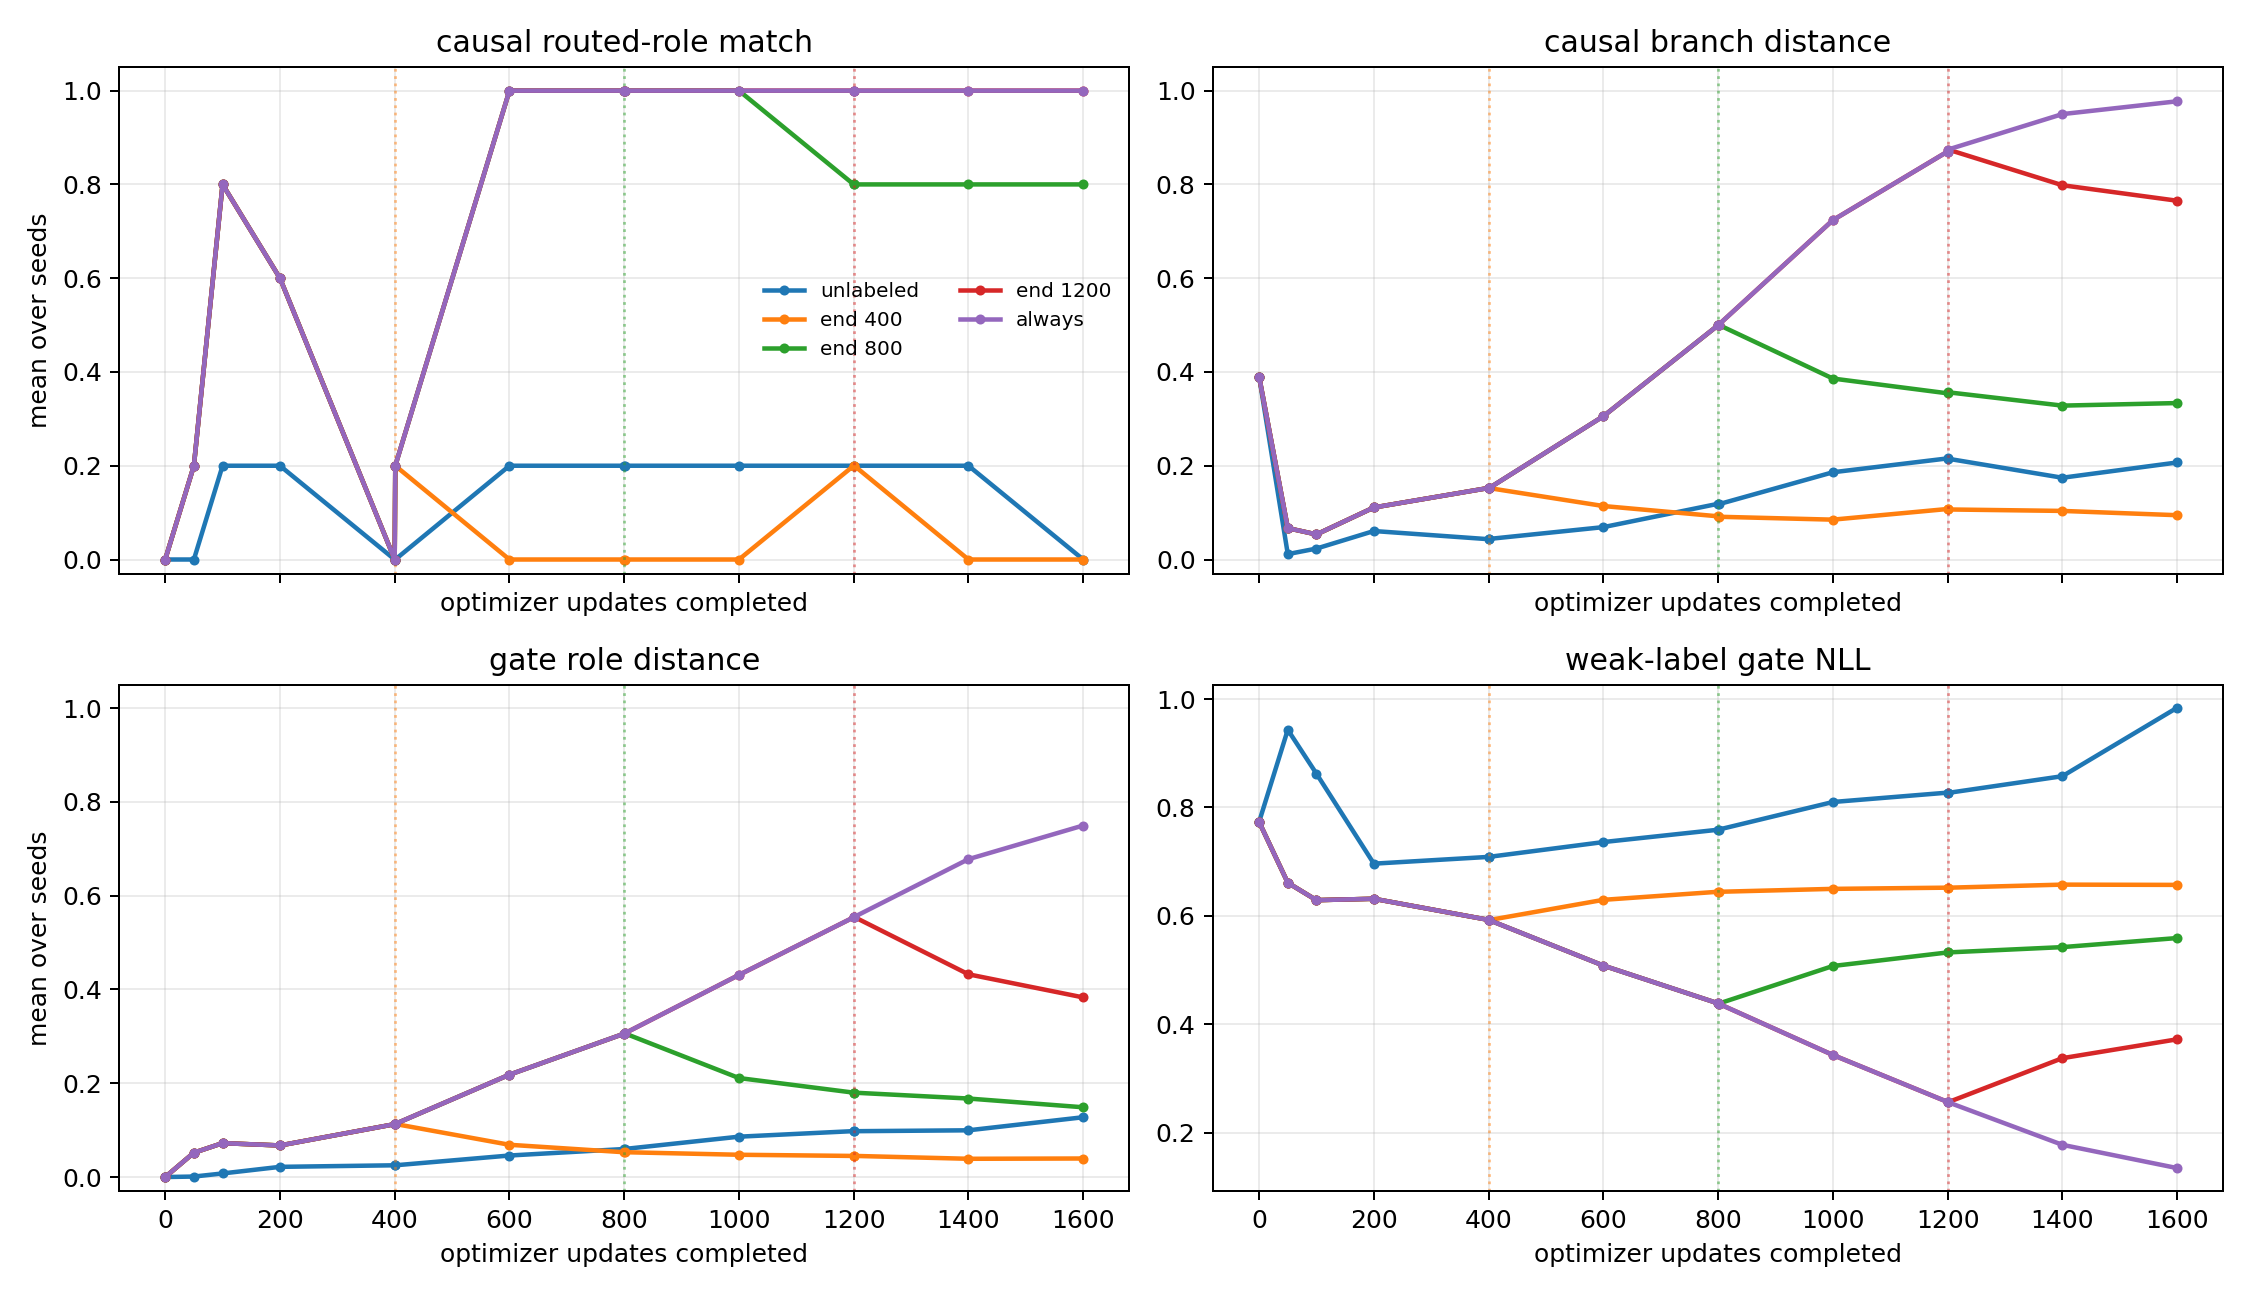
\includegraphics[height=0.70\textheight,keepaspectratio]{figures/router_trajectory_metrics.png}
  \end{center}

  \small
  Dotted vertical lines mark label-removal steps. The key transition is between
  step 400 and step 600: gates are already aligned, but causal branch modularity
  appears only under continued labels.
\end{frame}

\begin{frame}{Step 400 Is Not Enough}
  \small
  \begin{center}
  \begin{tabular}{lrrrrr}
    \toprule
    Schedule / step & Gate match & Gate dist. & Causal match & Branch dist. & Ind. acc. \\
    \midrule
    end 400 / 400 & 1.00 & 0.1127 & 0.00 & 0.1525 & 0.9990 \\
    end 400 / 600 & 1.00 & 0.0688 & 0.00 & 0.1141 & 0.9994 \\
    end 400 / 1600 & 0.60 & 0.0395 & 0.00 & 0.0945 & 0.9992 \\
    \bottomrule
  \end{tabular}
  \end{center}

  \vspace{0.8em}
  By step 400, task performance and gate alignment are already high. Removing
  labels there prevents causal branch modularity from consolidating.
\end{frame}

\begin{frame}{Continued Labels Make The Causal Split}
  \small
  \begin{center}
  \begin{tabular}{lrrrr}
    \toprule
    Schedule / step & Gate dist. & Causal match & Branch dist. & Gate NLL \\
    \midrule
    end 800 / 400 & 0.1127 & 0.00 & 0.1525 & 0.5927 \\
    end 800 / 600 & 0.2183 & 1.00 & 0.3056 & 0.5085 \\
    end 800 / 800 & 0.3058 & 1.00 & 0.4996 & 0.4388 \\
    end 800 / 1600 & 0.1488 & 0.80 & 0.3337 & 0.5593 \\
    \bottomrule
  \end{tabular}
  \end{center}

  \vspace{0.8em}
  The causal split appears by step 600 if labels continue. After label removal
  at step 800, the split mostly persists but weakens.
\end{frame}

\begin{frame}{Late Removal Preserves A Stronger Split}
  \small
  \begin{center}
  \begin{tabular}{lrrrr}
    \toprule
    Schedule / step & Gate dist. & Causal match & Branch dist. & Gate NLL \\
    \midrule
    end 1200 / 1200 & 0.5539 & 1.00 & 0.8701 & 0.2571 \\
    end 1200 / 1600 & 0.3831 & 1.00 & 0.7652 & 0.3725 \\
    always / 1200 & 0.5539 & 1.00 & 0.8701 & 0.2571 \\
    always / 1600 & 0.7497 & 1.00 & 0.9773 & 0.1351 \\
    \bottomrule
  \end{tabular}
  \end{center}

  \vspace{0.8em}
  Removing labels after a strong causal split preserves top-branch assignment,
  but continuous labels keep strengthening separation.
\end{frame}

\begin{frame}{Interpretation}
  \textbf{Result}
  \begin{itemize}
    \item Gate alignment is not sufficient evidence of functional modularity.
    \item The gate becomes role-aligned before the branches become causally
    separable.
    \item Branch modularity consolidates later under sustained role-aligned
    routing pressure.
  \end{itemize}

  \vspace{0.8em}
  \textbf{Caveat}
  \begin{itemize}
    \item Early routed-match values before the task is solved should not be
    interpreted strongly. The decision-relevant comparison is step 400 onward,
    when both roles have near-perfect accuracy.
  \end{itemize}
\end{frame}

\begin{frame}{Project-Level Update}
  The toy evidence now supports a causal-consolidation framing:

  \vspace{0.8em}
  \begin{center}
  \textit{Structural routing plus role-informative training pressure can produce
  functional branch modularity, but the branch computation lags behind gate
  alignment.}
  \end{center}

  \vspace{0.8em}
  The paper-facing question becomes:

  \vspace{0.5em}
  \begin{center}
  \textit{Under what training signals and time windows does structural
  modularity become causal functional modularity?}
  \end{center}
\end{frame}

\begin{frame}{Decision And Next Step}
  \textbf{Decision.} The current toy branch is coherent enough. Stop broad toy
  sweeps of router regularizers and anneal times.

  \vspace{0.8em}
  \textbf{Next step.} Move to a less hand-designed routed attention setting or a
  small real transformer task:
  \begin{itemize}
    \item keep role probes separate from causal branch-ablation or patching;
    \item test whether gate alignment again precedes causal modularity;
    \item compare structural routing, weak role labels, and unlabeled pressure.
  \end{itemize}
\end{frame}

\begin{frame}{Provenance}
  \small
  \textbf{Source files}
  \begin{itemize}
    \item \texttt{scripts/toy\_branch\_isolation\_intervention.py}
    \item \texttt{scripts/analyze\_router\_trajectory\_experiment.py}
    \item \texttt{doc/phase3\_toy\_router\_trajectory.md}
  \end{itemize}

  \vspace{0.4em}
  \textbf{Copied data in this deck folder}
  \begin{itemize}
    \item \texttt{data/trajectory\_by\_step.csv}
    \item \texttt{data/trajectory\_rows.csv}
    \item \texttt{figures/router\_trajectory\_metrics.png}
  \end{itemize}

  \vspace{0.4em}
  \textbf{Rebuild}
  \begin{itemize}
    \item \texttt{python3 -u scripts/analyze\_router\_trajectory\_experiment.py}
    \item \texttt{python3 .../compile\_latex\_deck.py presentations/2026-05-22-1745-router-trajectory/router\_trajectory\_checkpoint.tex}
  \end{itemize}
\end{frame}

\end{document}
